\chapter{Síntesis de software para GNC embebido}
\label{ch:especifico2}

En el capítulo \ref{ch:especifico1}, se realizó la selección de la tarjeta de desarrollo ZedBoard, además de esto uno de los requerimientos que se tomó en cuenta fue la compatibilidad de esta con el flujo de trabajo de Yocto Project.

\begin{figure}[h!]
    \centering
    \includegraphics[width=0.48\textwidth]{fig/especifico_2/Diagrama general del proyecto.pdf}
    \caption{Diagrama general del flujo de trabajo propuesto}
    \label{fig:diagrama_flujo_trabajo}
\end{figure}

En este capítulo se establecieron los flujos de trabajo para el prototipado de algoritmos de control, orientación y navegación para aplicaciones espaciales. Esto mediante la implementación de un caso de estudio básico. En la Figura \ref{fig:diagrama_flujo_trabajo}, se tomó un modelo de sistema de control, el cual debía implementar en MATLAB Simulink por medio de los bloques del sistema. 

Seguido de esto se realizó un ajuste de parámetros con el objetivo que el mismo opere dentro de las condiciones esperadas, una vez ajustado el sistema, se ingresó el modelo al flujo de trabajo de Simulink Coder, el cual nos dio como salida el código base y las herramientas de construcción requeridas para poder compilar el archivo ejecutable, cabe destacar que la compilación que se llevo a cabo fue cruzada, esta nos permitio compilar los archivos en un sistema distinto al objetivo. 

Finalmente se ingresó el archivo binario generado al flujo de trabajo de EmbedSynthGNC, el cual, se encargara de dar como salida un sistema de archivos de arranque y el sistema de directorios listos para implementar en la plataforma de desarrollo.


\section{Creación de los entornos de desarrollo}

En esta sección se describen los pasos desarrollados para la creación de los entornos de desarrollo utilizados en este proyecto. En el mismo se incluye la información del hardware y software utilizado, además de las versiones de los sistemas para cada una de las implementaciones. Cabe destacar que el computador anfitrión donde se implementaron estos entornos de desarrollo tiene las siguientes características:

\begin{itemize}
    \item Procesador Intel i9 - 13900k 
    \item Almacenamiento 1 TB
    \item Memoria 16 GB
    \item Video Nvidia RTX4060Ti
\end{itemize}

\subsection{MATLAB}\label{subsec:generacion_entorno_matlab}

Para el entorno de MATLAB se utilizó como sistema operativo Windows 11, en su versión de 64 bits, se destinó a este sistema operativo un espacio en disco de 500 GB, en el cual se instalaron los programas requeridos para la generación de contenido y el análisis de datos. La versión utilizada es MATLAB 2024b por medio de una licencia de prueba de la versión full, la cual nos permitió generar y probar el contenido necesario para los casos de uso a tratar. Por otro lado, para el análisis y procesamiento de datos se utilizó Python 3.12.3.

\begin{figure}[h!]
    \centering
    \includegraphics[width=0.5\textwidth]{fig/especifico_2/Entorno_windows}
    \caption{Diagrama para generar el entorno de MATLAB}
    \label{fig:diagrama_entorno_matlab}
\end{figure}

Según la Figura \ref{fig:diagrama_entorno_matlab}, para la generación de este entorno de trabajo primeramente se debe realizar la instalación de Python 3.12.3 y seguido de esto la instalación de MATLAB con las herramientas requeridas. Finalmente se instaló GCC en su versión 6.3.0.

Como primer paso se realizó la descarga de Visual Studio desde \href{https://code.visualstudio.com/sha/download?build=stable&os=win32-x64-user}{este enlace}, esto con el fin de poder hacer uso de Jupyter Notebook para el análisis de datos, además de esto se descargó Python en su versión 3.12.3 desde esta \href{https://www.python.org/ftp/python/3.12.3/python-3.12.3-amd64.exe}{dirección}. 


\begin{figure}[htbp]
    \centering
    \begin{subfigure}[b]{0.45\textwidth}
        \centering
        \includegraphics[width=\textwidth]{fig/especifico_2/Ambiente_matlab/instalacion_python.pdf}
        \caption{Menú de instalación de Python}
        \label{fig:menu_python}
    \end{subfigure}
    \hfill
    \begin{subfigure}[b]{0.45\textwidth}
        \centering
        \includegraphics[width=\textwidth]{fig/especifico_2/Ambiente_matlab/opciones_adicionales_python.pdf}
        \caption{Menú de instalación opcional}
        \label{fig:menu_python_adicionales}
    \end{subfigure}
    \caption{Instalación Python}
    \label{fig:menu_python_adicionales_2}
\end{figure}


Una vez descargados estos programas se realizó la instalación de los mismos, primeramente se instaló Python, el cual, según la Figura \ref{fig:menu_python} se seleccionó la opción para agregar Python al directorio PATH, esto con el fin de instalar los entornos y librerías requeridas. Seguido de esto se debe selecciono la opción de instalación personalizada (Customize installation) para poder agregar las características que se mostraron en la Figura \ref{fig:menu_python_adicionales}. 
\newpage

\begin{figure}[htbp]
    \centering
    \begin{subfigure}[b]{0.45\textwidth}
        \centering
        \includegraphics[width=\textwidth]{fig/especifico_2/Ambiente_matlab/instalacion_vs_code.pdf}
        \caption{Menú de instalación de VS Code}
        \label{fig:menu_vscode}
    \end{subfigure}
    \hfill
    \begin{subfigure}[b]{0.45\textwidth}
        \centering
        \includegraphics[width=\textwidth]{fig/especifico_2/Ambiente_matlab/opciones_adicionales_vs_code.pdf}
        \caption{Menú de instalación de VS Code (opcionales)}
        \label{fig:menu_vscode_adicionales}
    \end{subfigure}
    \caption{Instalación VSCode}
    \label{fig:menu_vscode_2}
\end{figure}


Una vez concluida la instalación de Python de continuo con VS Code, el cual como se observa en la Figura \ref{fig:menu_vscode}, se aceptaron los términos y condiciones del programa y en el siguiente menú se seleccionaron las opciones marcadas en la Figura \ref{fig:menu_vscode_adicionales}.

Finalmente se realizó la descarga de MATLAB  por medio de \href{https://matlab.mathworks.com/}{este enlace}. COmo un paso adicional se tuvo que registrar una cuenta y esto habilito la descarga de la versión de prueba que tiene una durabilidad de 30 días. Dentro de la instalación es importante mencionar que se solicitaron todas las herramientas dentro del periodo de prueba, pero las herramientas que resultaron esenciales para el desarrollo del mismo fueron las siguientes:

\begin{itemize}
    \item MATLAB Simulink
    \item MATLAB Coder
\end{itemize}

Además, se instaló la herramienta GCC en su versión 6.3.0, el cual es el compilador de código C, este se utilizó para compilar el código y probar que el mismo funcione de la forma esperada; cabe destacar, que este no es el compilador cruzado, este compilador se encargó de generar un archivo binario el cual se probo en el sistema Windows, esto con el fin de realizar correcciones más eficientes al sistema.

\subsection{Implementación de contenedores}\label{sec:entorno_en_contenedores}

En la elaboración del proyecto se decantó por el uso de contenedores, como se menciona en \ref{sec:containers}, estos permitieron encapsular todas las dependencias y configuraciones necesarias para ejecutar una aplicación. Esto aseguro que la aplicación funcione de manera consistente en diferentes entornos, ya sea durante el desarrollo. 

Cada contenedor opera de forma independiente, lo que permite ejecutar múltiples aplicaciones en el mismo sistema sin interferencias. Este aislamiento redujo significativamente el riesgo de conflictos entre diferentes versiones de software y dependencias, lo que se tradujo en un entorno más estable y predecible. Los contenedores se construyeron en el computador anfitrión en un sistema operativo Linux en su versión 22.04 LTS.

\subsubsection{Comandos utilizados para la creación y gestión de contenedores}\label{subsec:manejo_de_contenedores}


\begin{lstlisting}[language=bash, caption={Instalacion de docker, Linux}, label=lst:install_docker]
    sudo apt install docker.io
\end{lstlisting}

Mediante el uso de \ref{lst:install_docker}, se realizó la instalación de docker.io, el cual como se menciona en \ref{sec:containers}, es una plataforma que permite la creación, despliegue y gestión de aplicaciones en contenedores. 

\begin{lstlisting}[language=bash, caption={Instalacion de Ubuntu 20.04, Linux}, label=lst:install_20_04_ubuntu]
    sudo docker run -it ubuntu:20.04 /bin/bash
\end{lstlisting}

Por medio del comando \ref{lst:install_20_04_ubuntu} se realizó la construcción del contenedor. Este último comando se encargó de descargar la imagen de Ubuntu 20.04, crea y ejecuta un contenedor en modo interactivo además de proporcionar acceso al terminal del contenedor, donde se ejecutan comandos como si fuera una máquina virtual con Ubuntu 20.04. Este contenedor se utilizó para realizar la compilación cruzada, se tomó la decisión de utilizar Ubuntu 20.04, ya que esta versión contiene la versión de GCC que satisface los requerimientos impuestos por otros flujos de trabajo.

\begin{lstlisting}[language=bash, caption={Instalacion de Ubuntu 16.04, Linux}, label=lst:install_16_04_ubuntu]
    sudo docker run -it ubuntu:16.04 /bin/bash
\end{lstlisting}

Por otro lado, el comando \ref{lst:install_16_04_ubuntu}, genero el contenedor que fue utilizado para la implementación del flujo de trabajo de Yocto Project, cabe destacar que se utilizo Ubuntu 16.04, ya que, es la versión que cumple con los requerimientos del flujo de trabajo de Yocto, esto se debe a que al trabajar con Yocto Zeus y este ser desarrollado en el año 2019, esta era la versión de Ubuntu estable para la fecha. 

\begin{lstlisting}[language=bash, caption={Lista de contenedores del sistema, Docker}, label=lst:docker_basics_ps-a]
    sudo docker ps -a
\end{lstlisting}

\begin{figure}[h!]
    \centering
    \includegraphics[width=0.85\textwidth]{fig/especifico_2/retornos_de_comandos/sudo_docker_ps_a.pdf}
    \caption{Retorno del comando \ref{lst:docker_basics_ps-a}}
    \label{fig:sudo_docker_ps_a}
\end{figure}

Una vez fueron generados los dos contenedores, fueron consultados mediante el comando \ref{lst:docker_basics_ps-a}, este se encarga de devolver una lista como en la Figura \ref{fig:sudo_docker_ps_a}, donde se observó de izquierda a derecha las columnas denominadas: Container ID, el cual es el identificador del contenedor, este valor se utilizó para referirse al contenedor para las operaciones que se realizaron fuera del entorno, también se muestra la Imagen que el contenedor tiene instalada, el comando de creación del mismo, la creación del contenedor, el status, los puertos definidos y el Nombre.

Para efectos de este proyecto se tomó importancia solamente a las columnas de (Container ID) e (Image).

\begin{lstlisting}[language=bash, caption={Iniciar un contenedor, Docker}, label=lst:docker_basics_start]
    sudo docker start <ID del contenedor>
\end{lstlisting}

\begin{figure}[h!]
    \centering
    \includegraphics[width=0.85\textwidth]{fig/especifico_2/retornos_de_comandos/sudo_docker_start.pdf}
    \caption{Retorno del comando \ref{lst:docker_basics_start}}
    \label{fig:sudo_docker_start}
\end{figure}

Por medio del comando \ref{lst:docker_basics_start} se inició el contenedor deseado, esto siempre dependerá del ID que se coloque, tras la ejecución de este comando la salida del mismo se observa en la Figura \ref{fig:sudo_docker_start}.

\begin{lstlisting}[language=bash, caption={Ingresar a un contenedor, Docker}, label=lst:docker_basics_init]
    sudo docker exec -it <ID del contenedor> \bin\bash
\end{lstlisting}

\begin{figure}[h!]
    \centering
    \includegraphics[width=0.85\textwidth]{fig/especifico_2/retornos_de_comandos/sudo_docker_init.pdf}
    \caption{Retorno del comando \ref{lst:docker_basics_init}}
    \label{fig:sudo_docker_init}
\end{figure}

Finalmente, para la ejecución del contenedor en terminal se utilizó el comando \ref{lst:docker_basics_init}, este se encargó de acceder a la terminal del contenedor deseado. Como se observa en la Figura \ref{fig:sudo_docker_init} ya la terminal se encontraba ejecutando el contenedor construido bajo el ID del contenedor "1420fedd3067".

Una vez generados los contenedores, se procedió a construir el entorno de desarrollo requerido dentro de los mismos.
\newpage

\subsubsection{Contenedor para compilación Cruzada}\label{subsec:generacion_entorno_xcompile}

\begin{figure}[htbp]
    \centering
    \includegraphics[width=0.4\textwidth]{fig/especifico_2/diagrama_compilador_cruzado.pdf}
    \caption{Diagrama para la elaboración del entorno para compilación cruzada}
    \label{fig:cross_compile_diagram}
\end{figure}

Para la compilación de los archivos se elaboró un entorno para compilación cruzada, esto se debe a que el archivo se compiló para la ejecución en la plataforma de desarrollo seleccionada, es por esto que para la preparación del entorno se siguieron los pasos de la Figura \ref{fig:cross_compile_diagram}


\begin{lstlisting}[language=bash, caption={Instalacion del compilador cruzado, Contenedor}, label=lst:cross_compiler]
    sudo apt install gcc-arm-linux-gnueabihf
\end{lstlisting}

\begin{lstlisting}[language=bash, caption={Instalacion de CMake, Contenedor}, label=lst:cmake]
    sudo apt install cmake
\end{lstlisting}

\begin{lstlisting}[language=bash, caption={Instalacion de build essential, Contenedor }, label=lst:build_essential]
    sudo apt install build-essential
\end{lstlisting}

Primeramente se instaló el compilador cruzado, para efectos de este trabajo fue arm-linux-gnueabihf-gcc, esto se implementó mediante el comando \ref{lst:cross_compiler}. Seguido de esto se instaló CMake el cual es una herramienta de construcción multiplataforma y de código abierto que se utilizó para gestionar la construcción de software, el mismo se instaló mediante el comando \ref{lst:cmake}. Finalmente también se instaló build-essential las cuales son herramientas que nos ayudaron a compilar el programa generado, esta instalación se logró mediante el comando mostrado en \ref{lst:build_essential}. Luego de estas tres instalaciones quedo preparado el entorno para la compilación cruzada. 

\newpage

\subsubsection{Contenedor para Yocto Project}\label{subsec:generacion_entorno_yocto}

\begin{figure}[h!] 
    \centering
    \includegraphics[width=0.85\textwidth]{fig/especifico_2/diagrama_de_entorno_yocto_project.pdf}
    \caption{Diagrama para la elaboración del entorno para Yocto Project}
    \label{fig:yocto_enviroment_diagram_figure}
\end{figure}

El contenedor para Yocto Project, fue en el cual se llevo cabo la construcción de la imagen utilizada en la plataforma de desarrollo, para esto se requirio la instalación de algunas dependencias las cuales se observan en la Figura \ref{fig:yocto_enviroment_diagram_figure}.



\subsubsection{Creación de un usuario no root}

Para el uso del marco de trabajo de Yocto se genero un usuario no root, esto principalmente por razones de seguridad y manejo adecuado de permisos.

\begin{lstlisting}[language=bash, caption={Generacion de usuario no root, Linux}, label=lst:no_root_user]
    apt - get install -y sudo
    useradd - ms/bin/bash myuser
    echo "myuser:password" | chpasswd
    usermod - aG sudo myuser
\end{lstlisting}

De forma que según el comando \ref{lst:no_root_user}, en la primera línea se realizó la instalación de sudo, esto con el objetivo de poder ejecutar comandos con privilegios de administrador sin tener que iniciar sesión como usuario root, seguido de esto en la segunda línea se agregó el usuario denominado (myuser), en la tercera línea se generó una contraseña para este usuario la cual se definió como (chpasswd), finalmente se agregó en el archivo usermod el nuevo usuario el cual, mediante el uso del comando sudo tiene acceso a los privilegios de administrador. 

\begin{lstlisting}[language=bash, caption={Iniciar usuario no root, Linux}, label=lst:no_root_user_log]
    su - myuser
\end{lstlisting}

Cada vez que se inicie el contenedor siempre lo hara como usuario root. Para poder iniciar con el usuario no root generado en \ref{lst:no_root_user}, se debe hacer uso del comando que se muestra en \ref{lst:no_root_user_log}, el cual se encarga de iniciar el entorno bajo el usuario llamado (myuser). Cada vez que se realice alguna instalación o procedimiento que requiera permisos de administrador se deberá de ingresar la contraseña.

\subsubsection{Yocto Project}

Como se observó en \ref{subsec:yocto}, Yocto presenta flexibilidades a la hora de configurar un sistema permitiendo al desarrollador seleccionar paquetes específicos y personalizar el sistema operativo.

\begin{lstlisting}[language=bash, caption={Requerimientos Yocto Zeus, Linux}, label=lst:yocto_requirements]
    sudo apt - get install gawk wget git - core diffstat unzip texinfo
    gcc - multilib build - essential chrpath socat cpio python python3
    python3 - pip python3 - pexpect xz - utils debianutils 
    iputils - ping python3 - git python3 - jinja2 
    libegl1 - mesa libsdl1 .2 - dev pylint3 xterm
\end{lstlisting}

Para que el mismo funcionara de forma correcta se debieron de instalar los requerimientos del marco de trabajo \ref{lst:yocto_requirements}.

\begin{lstlisting}[language=bash, caption={Version de Yocto}, label=lst:yocto_clone]
    git clone -b zeus https://git.yoctoproject.org/git/poky
    cd poky
\end{lstlisting}

\begin{lstlisting}[language=bash, caption={BSP para Zedboard}, label=lst:yocto_zedboard]
    git clone -b zeus https://github.com/Xilinx/meta-xilinx
    git clone -b zeus https://github.com/openembedded/meta-openembedded.git
\end{lstlisting}

La versión de Yocto que se utilizo es Yocto Zeus, ya que esta versión es la que contiene soporte para la tarjeta de desarrollo ZedBoard, los archivos de esta versión se cloraon de \ref{lst:yocto_clone}. Una vez clonado el repositorio se debe ingreso al directorio (poky) y adicionalmente se clonó, dentro del mismo, el repositorio \ref{lst:yocto_zedboard} el cual contiene la versión de paquete de soporte para la tarjeta ZedBoard, esto con el objetivo de generar una imagen para la tarjeta de desarrollo.

\begin{lstlisting}[language=bash, caption={Configuraciones adicionales, Yocto}, label=lst:aditional_config]
    source oe - init - build - env
    
    echo "MACHINE ??=\"zedboard-zynq7\"" >> conf/local.conf
    echo "IMAGE_FEATURES +=\"package-management\"" >> conf/local.conf
    echo "DISTRO_HOSTNAME =\"zynq\"" >> conf/local.conf
    
    bitbake-layers add-layer ../meta-xilinx/meta-xilinx-bsp/
    bitbake-layers add-layer ../meta-openembedded/meta-oe/
\end{lstlisting}

Una vez clonados los repositorios se continuó con algunas configuraciones adicionales que se debían de realizar, con el fin de configurar correctamente el entorno de trabajo, estas se enlistaron en \ref{lst:aditional_config}. La primera línea se encargó de configurar el entorno de trabajo dentro del directorio llamado (build). Dentro del entorno de trabajo generado en (build) en el directorio llamado (conf) se encontraron archivos como el local.conf este es un archivo de configuración utilizado por el sistema de compilación BitBake. Este archivo está escrito en lenguaje de configuración de BitBake, define aspectos importantes como la arquitectura del objetivo, la distribución del sistema las imágenes a crear y las herramientas utilizadas, además de incluir rutas adicionales a capas de Yocto o bien a configuraciones específicas de las recetas. 

Además de esto también nos encontramos con el archivo llamado bblayers.conf, este al igual que local.conf, es un archivo de configuración de BitBake que define las capas que se utilizan durante el proceso de compilación. En este como se mencionó anteriormente se encuentran las rutas de las diferentes capas que el sistema de compilación de Yocto debe usar. Estas capas contienen las recetas y los archivos de configuración que controlan la compilación de paquetes, imágenes y el sistema operativo en general. Cabe destacar que el orden en el que se listan las capas puede ser importante, ya que capas más específicas pueden sobreescribir las configuraciones o recetas de capas más generales.

Una vez comprendidos estos conceptos la línea 3 de \ref{lst:aditional_config} se encargo de agregar la máquina, que en nuestro caso sería la tarjeta de desarrollo ZedBoard de Avnet, la línea 4 se habilitó la administración de paquetes, esto quiere decir que se asegura que el sistema que se está construyendo incluirá las herramientas necesarias para gestionar paquetes (como instalar, actualizar o eliminar) después de que el sistema haya sido desplegado. La línea 4 se encargó de establecer el nombre del anfitrión, el sistema operativo generado tendrá el nombre de anfitrión configurado como zynq. Por otro lado, la línea 7 y 8 se encargaron de agregar las capas al archivo de bblayers.conf.

Finalizada la configuración básica de los entornos de trabajo se sigue con las siguientes secciones en donde se desarrollaron los casos de estudio con el objetivo de demostrar el funcionamiento del flujo de trabajo propuesto en la Figura \ref{fig:diagrama_flujo_trabajo}.

\newpage

\section{Caso de estudio 1 - Filtro Básico en MATLAB}

Como caso de estudio se seleccionó una aplicación la cual permitió realizar una comparación de resultados antes y después del procesamiento de datos, es por esto que se decidió implementar un filtro básico de tipo paso bajo haciendo uso de los bloques de MATLAB Simulink. 

\begin{figure}[h!]
    \centering
    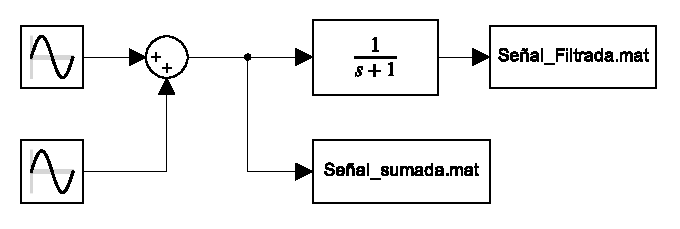
\includegraphics[width=0.5\textwidth]{fig/especifico_2/CASO_ESTUDIO_FILTRO/Diagrama matlab simulink.pdf}
    \caption{Diagrama caso de estudio 1 - Filtro Básico}
    \label{fig:diagrama_matlab_simulink}
\end{figure}

Para la construcción del caso de estudio sé propuso el diagrama de la Figura \ref{fig:diagrama_matlab_simulink}, donde para su construcción se llevaron a cabo los siguientes pasos.

\begin{figure}[h!]
    \centering
    \includegraphics[width=0.8\textwidth]{fig/especifico_2/CASO_ESTUDIO_FILTRO/libbroswer_0.pdf}
    \caption{Librería de bloques}
    \label{fig:lib_bloq}
\end{figure}

Primeramente se tuvo acceso a la librería de bloques, la misma se pudo encontrar en la ubicación que se muestra en la Figura \ref{fig:lib_bloq}, a esta se accedió haciendo click en el icono que se encuentra resaltado en la Figura anteriormente mencionada.



\begin{figure}[h!]
    \centering
    \includegraphics[width=0.5\textwidth]{fig/especifico_2/CASO_ESTUDIO_FILTRO/sinewave_0.pdf}
    \caption{Librería de bloques - generador de onda senoidal}
    \label{fig:lib_bloq_sine}
\end{figure}

Una vez en la librería de bloques, como se observa en la Figura \ref{fig:lib_bloq_sine} se ingreso en el buscador marcado en color rojo la palabra clave del bloque que se desea buscar, para este caso se buscó el generador de onda seno del cual se ocupan dos bloques. 

\begin{figure}[htbp]
    \centering
    \begin{subfigure}[b]{0.45\textwidth}
        \centering
        \includegraphics[width=0.7\textwidth]{fig/especifico_2/CASO_ESTUDIO_FILTRO/sinewave_1.pdf}
        \caption{Generador de onda seno 1}
        \label{fig:sine_gen_01}
    \end{subfigure}
    \hfill
    \begin{subfigure}[b]{0.45\textwidth}
        \centering
        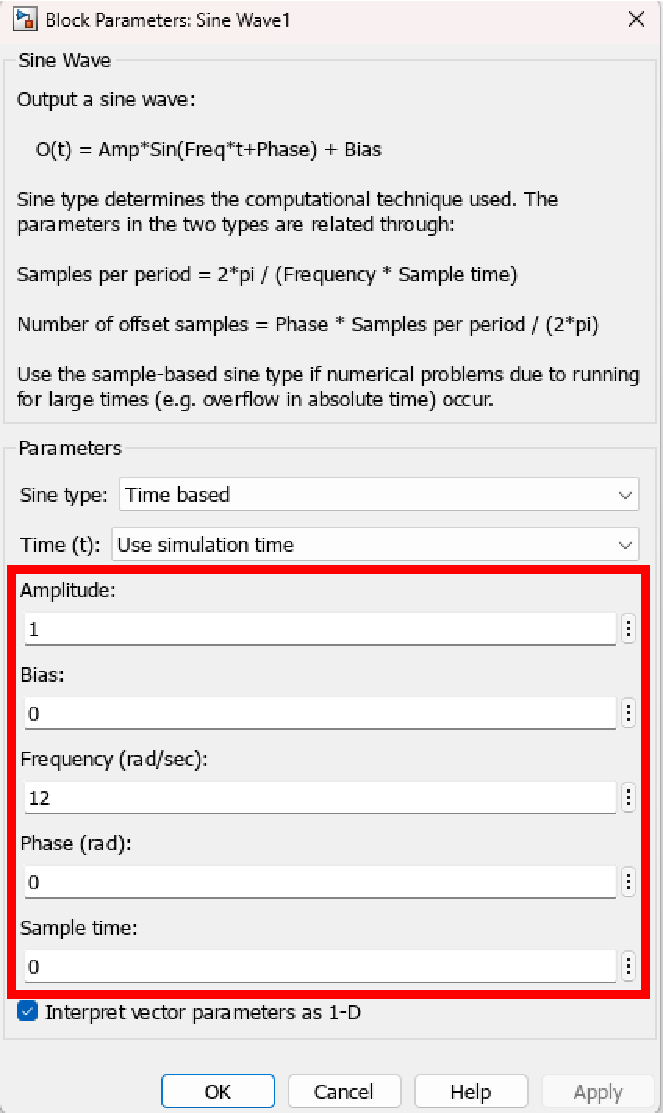
\includegraphics[width=0.7\textwidth]{fig/especifico_2/CASO_ESTUDIO_FILTRO/sinewave_2.pdf}
        \caption{Generador de onda seno 2}
        \label{fig:sine_gen_02}
    \end{subfigure}
    \caption{Configuración de los generadores de onda senoidal}
    \label{fig:sine_wave_generators_config}
\end{figure}

Para la configuración de los generadores de onda senoidales se siguieron las configuraciones que se muestran en la Figura \ref{fig:sine_wave_generators_config}, de forma que al primer bloque generador de onda seno se le coloco la configuración que se muestra en \ref{fig:sine_gen_01} y al segundo la que se muestra en \ref{fig:sine_gen_02}. De esta forma quedaron configurados los bloques encargados de generar las ondas según los parámetros indicados.


\begin{figure}[h!]
    \centering
    \includegraphics[width=0.5\textwidth]{fig/especifico_2/CASO_ESTUDIO_FILTRO/sum_0.pdf}
    \caption{Librería de bloques - sumador de señales}
    \label{fig:lib_bloq_sum}
\end{figure}

\begin{figure}[h!]
    \centering
    \includegraphics[width=0.5\textwidth]{fig/especifico_2/CASO_ESTUDIO_FILTRO/sum_1.pdf}
    \caption{Configuración del bloque sumador de señales}
    \label{fig:lib_bloq_sum_conf}
\end{figure}


Seguido de esto se implementó el bloque sumador el cual se muestra en la Figura \ref{fig:lib_bloq_sum}, este mismo se configuró como se muestra en la Figura \ref{fig:lib_bloq_sum_conf}, este bloque nos ayudó a sumar las dos señales senoidales, ya que al sumar ondas de diferentes frecuencias, se genera un fenómeno llamado modulación, donde la onda resultante presenta un patrón que varía en el tiempo.

\begin{equation}
    y(t) = \sin(t) + \sin(12t)
    \label{eq:funcion_de_suma_de_ondas}
\end{equation}

Por otro lado la función de transferencia utilizada en el filtro fue:

\begin{equation}
    H(S) = \frac{1}{S+1}
    \label{eq:funcion_de_transferencia_filtro}
\end{equation}

\newpage

\begin{figure}[htbp]
    \centering
    \begin{subfigure}[b]{0.45\textwidth}
        \centering
        \includegraphics[width=0.9\textwidth]{fig/especifico_2/CASO_ESTUDIO_FILTRO/Transfer_func.pdf}
        \caption{Librería de bloques - función de \\ transferencia}
        \label{fig:lib_bloq_transfer_func}
    \end{subfigure}
    \hfill
    \begin{subfigure}[b]{0.45\textwidth}
        \centering
        \includegraphics[width=0.7\textwidth]{fig/especifico_2/CASO_ESTUDIO_FILTRO/Transfer_func_1.pdf}
        \caption{Configuración del bloque función de \\ transferencia}
        \label{fig:lib_bloq_transfer_func_conf}
    \end{subfigure}
    \caption{Bloque función de transferencia}
    \label{fig:lib_bloq_transfer_func_all}
\end{figure}

Como se observa en la Figura \ref{fig:lib_bloq_transfer_func_all}, a la izquierda \ref{fig:lib_bloq_transfer_func} el bloque de función de transferencia en la librería de bloques, por otro lado a la derecha en \ref{fig:lib_bloq_transfer_func_conf},  la configuración utilizada en el mismo, esto con el objetivo de ejecutar la función que se muestra en \ref{eq:funcion_de_transferencia_filtro}. De esta forma al aplicar el filtro a la señal compuesta,  la onda $\sin(t)$ paso a través del filtro con poca atenuación, mientras que la onda $\sin(12t)$ fue significativamente atenuada debido a su  alta frecuencia.

Estos bloques mencionados anteriormente se colocan como se muestra en la Figura \ref{fig:diagrama_matlab_simulink} de modo que se obtuvo como salida del sistema dos archivos, uno llamado señal sumada el cual contenía los datos crudos de la modulación de las dos señales senoidales y otro denominado señal filtrada el cual contenía los datos de la señal filtrada por la función de transferencia.

\newpage

\subsection{Simulación del caso de estudio en MATLAB Simulink}\label{subsec:simulacion_caso_de_estudio}

\begin{figure}[h!]
    \centering
    \includegraphics[width=0.5\textwidth]{fig/especifico_2/CASO_ESTUDIO_FILTRO/scope_0.pdf}
    \caption{Librería de bloques - gráfico}
    \label{fig:lib_bloq_graph}
\end{figure}

Para la simulación del caso de estudio de la Figura \ref{fig:diagrama_matlab_simulink} se requirio un bloque adicional, el cual se encargó de mostrar de forma grafica los resultados de la ejecución, el mismo se observa en la Figura \ref{fig:lib_bloq_graph}.

\begin{figure}[h!]
    \centering
    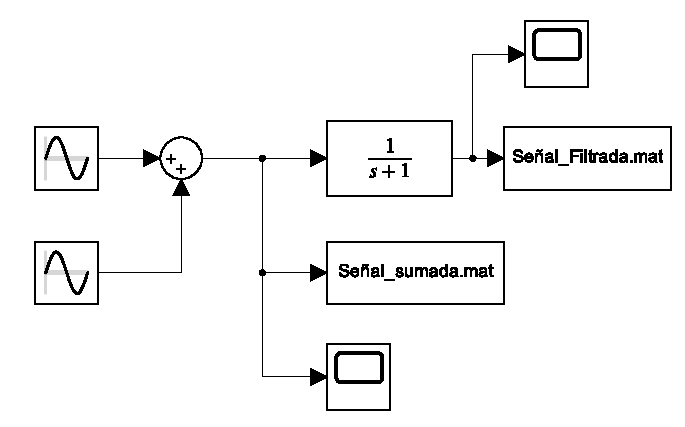
\includegraphics[width=0.5\textwidth]{fig/especifico_2/CASO_ESTUDIO_FILTRO/Diagrama matlab simulink scope.pdf}
    \caption{Diagrama MATLAB Simulink para poder observar las salidas}
    \label{fig:diagrama_matlab_simulink_graficos}
\end{figure}

De esta forma el diagrama de la Figura \ref{fig:diagrama_matlab_simulink}, se colocaron dos bloques de gráfico en el diagrama según se muestra en la Figura \ref{fig:diagrama_matlab_simulink_graficos}, esto con el objetivo de poder observar las señales de salida en cada uno de los puntos de interés.


\newpage

\subsubsection{Resultados obtenidos con la ejecución de la simulación}


\begin{figure}[htbp]
    \centering
    \begin{subfigure}[b]{0.45\textwidth}
        \centering
        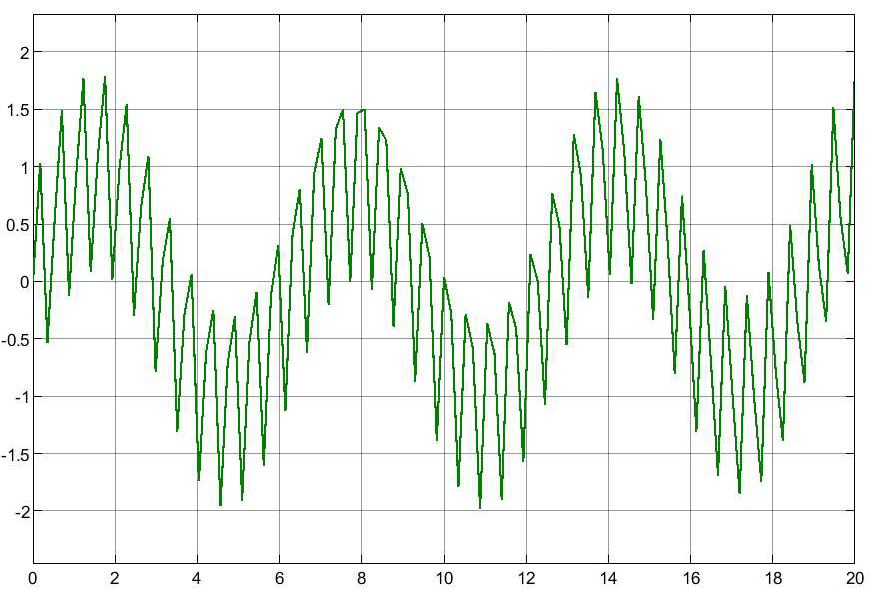
\includegraphics[width=\textwidth]{fig/especifico_2/onda_modulada.pdf}
        \caption{Ondas Moduladas}
        \label{fig:onda_modulada}
    \end{subfigure}
    \hfill
    \begin{subfigure}[b]{0.45\textwidth}
        \centering
        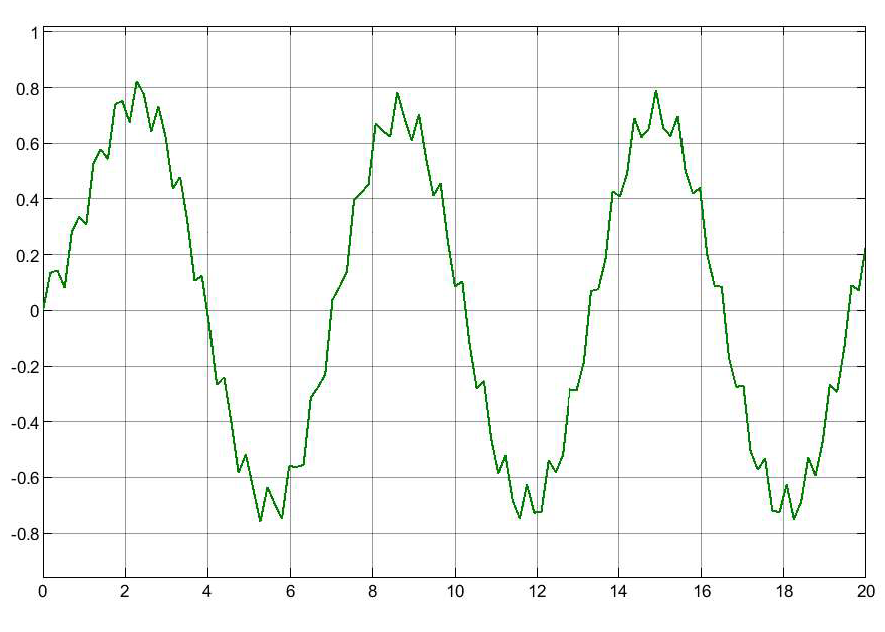
\includegraphics[width=\textwidth]{fig/especifico_2/onda_filtrada.pdf}
        \caption{Onda resultante luego de la función de transferencia}
        \label{fig:onda_filtrada}
    \end{subfigure}
    \caption{Salida simulada del diagrama mostrado en la Figura \ref{fig:diagrama_matlab_simulink_graficos}}
    \label{fig:salida_resultante_diagrama_graficos}
\end{figure}


En la Figura \ref{fig:onda_modulada} se observan la modulación de las dos señales senoidales, por otro lado, en \ref{fig:onda_filtrada} se observa la salida de la función de transferencia. Siendo la salida esperada de la función de transferencia, ya que al ser un filtro paso bajo atenúa las señales que estén por debajo de la frecuencia de corte, que para este filtro es de 1 $rad/s$. Como la señal compuesta contiene una onda seno con frecuencia de 1 $rad/s$ y otra con frecuencia de 12 $rad/s$ es posible observar aun componentes de la frecuencia atenuada.

\section{Flujo de trabajo de la aplicación de transformación de modelo a modelo}\label{sec:m2m_transformator}

Para poder cumplir con el objetivo de embeber el sistema, se utilizó de la herramienta MATLAB Simulink Coder. Como se menciona en \ref{sec:modelo2model}, a este tipo de aplicaciones se les conoce como transformadores de modelos, en este caso se empleo para lograr transformar el diagrama de control implementado en MATLAB Simulink en un código de lenguaje C, manteniendo de esta forma la estructura del modelo, pero realizando una adaptación al formato requerido, este convertidor de modelos garantizo la consistencia del modelo de control además de realizar la adaptación del mismo a las características de la tarjeta de desarrollo ZedBoard. Algunos de los parámetros que se pueden configurar en este transformador de modelos son: parámetros de la solución, implementación en hardware y generación de código.
\newpage

\begin{figure}[h!]
    \centering
    \includegraphics[width=0.4\textwidth]{fig/especifico_2/M2MT/model_2_model_diagram.pdf}
    \caption{Flujo de trabajo MATLAB Simulink Coder}
    \label{fig:m2m_matlab_simulink_coder}
\end{figure}

En la Figura \ref{fig:m2m_matlab_simulink_coder} se encuentra un diagrama que contempla los pasos a seguir en esta sección, los cuales se explican a lo largo de este capítulo, además, se definieron los parámetros a utilizar y el funcionamiento de estos dentro de la generación del código C.

\subsection{Simulink Coder}\label{subsec:simulink_coder}

Una vez comprobado el comportamiento del caso de estudio mediante la simulación, se procedió con la ejecución del flujo de trabajo de MATLAB Simulink Coder, esto con el fin de transformar el modelo generado en MATLAB Simulink a un modelo de lenguaje de programación C. Cabe destacar que para esta implementación se utilizó el diagrama de Figura \ref{fig:diagrama_matlab_simulink}, ya que, este solamente contenía como salida los archivos con los datos numéricos del sistema y no las salidas gráficas agregadas en \ref{subsec:simulacion_caso_de_estudio}.


\subsection{Definición de parámetros}

\begin{figure}[h!]
    \centering
    \includegraphics[width=0.8\textwidth]{fig/especifico_2/M2MT/paso_a_paso_mtmt/apps.pdf}
    \caption{Pestaña Aplicaciones}
    \label{fig:pestana_apps}
\end{figure}

\begin{figure}[h!]
    \centering
    \includegraphics[width=0.8\textwidth]{fig/especifico_2/M2MT/paso_a_paso_mtmt/c_code.pdf}
    \caption{Pestaña código C}
    \label{fig:pestana_c_code}
\end{figure}

\begin{figure}[h!]
    \centering
    \includegraphics[width=0.8\textwidth]{fig/especifico_2/M2MT/paso_a_paso_mtmt/configuration_parameters.pdf}
    \caption{Configuración de parámetros}
    \label{fig:pestana_config}
\end{figure}


Para la definición de parámetros, primero se abrió el programa MATLAB Simulink, una vez en el entorno se seleccionó la pestaña denominada Aplicaciones (APPS) como se muestra en la Figura \ref{fig:pestana_apps}. Se seleccionó la aplicación denominada Simulink Coder, con esta opción se abrió la pestaña llamada código C, (C CODE) como se pudo observar en la Figura \ref{fig:pestana_c_code}.

En la pestaña llamada código C, se seleccionó la opción de configuración de parámetros, en la Figura \ref{fig:pestana_c_code} se observa esta opción bajo el nombre de settings, cuando se ingresó esta opción se abrió una ventana emergente como la que se muestra en la Figura \ref{fig:pestana_config}, en la pestaña denominada Solver se proporcionaron los datos sobre el tiempo de ejecución de la prueba.

\subsubsection{Selección del procesador objetivo}

\begin{figure}[h!]
    \centering
    \includegraphics[width=0.8\textwidth]{fig/especifico_2/M2MT/paso_a_paso_mtmt/configuration_parameters_processor.pdf}
    \caption{Selección del procesador y la familia del procesador}
    \label{fig:pestana_config_procesador}
\end{figure}

En la pestaña llamada implementación de hardware (Hardware Implementation), se colocaron los datos de Fabricante del hardware (Device Vendor) el cual hace referencia al tipo de procesador que contiene la tarjeta de desarrollo, para nuestro caso se seleccionó ARM Compatible y el tipo de dispositivo (Device Type) correspondiente a la familia del procesador, la tarjeta de desarrollo ZedBoard cuenta con un procesador ARM Cortex-A de 32-bits, como se muestra en la Figura \ref{fig:pestana_config_procesador}.


\subsubsection{Selección del tipo de archivo de construcción}

Con los pasos anteriores se configuraron los parámetros de tiempo de operación y procesador de la tarjeta de desarrollo. En esta sección se configuró el tipo de archivo que se utilizó para la generación de los archivos binarios, como se debe realizar una compilación cruzada se eligió un tipo de archivo el cual nos permite compilar el código C para la ejecución del sistema sin importar el sistema operativo de la máquina anfitrión. 

Para esto, se seleccionó en la pestaña de generación de código (Code Generation) el kit de herramientas (Toolchain) denominado CMake como muestra en la Figura \ref{fig:pestana_config_output_file}, además de esto se marcó tanto la opción generar solamente el código (Generate code only), como empacar código y artefactos (Package code and artifacts), esta última opción nos generó como salida un archivo comprimido con todos los requerimientos de la aplicación.


\begin{figure}[h!]
    \centering
    \includegraphics[width=0.8\textwidth]{fig/especifico_2/M2MT/paso_a_paso_mtmt/configuration_output_file.pdf}
    \caption{Selección del tipo de archivo de construcción}
    \label{fig:pestana_config_output_file}
\end{figure}

\subsubsection{Generación de archivos de compilación}

Para la construcción de los archivos, se seleccionó la opción de generar código, como se observa en la Figura \ref{fig:pestana_c_code} bajo el nombre de (Build).

\begin{figure}[h!]
    \centering
    \includegraphics[width=0.8\textwidth]{fig/especifico_2/M2MT/paso_a_paso_mtmt/root_folder.pdf}
    \caption{Archivo comprimido en el directorio swap\_area}
    \label{fig:pestana_swap_area}
\end{figure}

\begin{lstlisting}[language=bash, caption={Copiar archivos al contenedor, Linux}, label=lst:copy_to_container]
    sudo docker cp /direccion/del/archivo 
    <id_de_contenedor>:/direccion/del/contenedor
\end{lstlisting}

\begin{lstlisting}[language=bash, caption={Copiar archivos del contenedor, Linux}, label=lst:copy_from_container]
    sudo docker cp <id_de_contenedor>:/direccion/del/contenedor
    /direccion/del/archivo
\end{lstlisting}

Seguido de esto copio el archivo comprimido generado en \ref{subsec:simulink_coder}, al contenedor con Ubuntu 16.04 generado en \ref{sec:entorno_en_contenedores}. Para esto se colocó el archivo comprimido en un directorio llamado swap\_area, como se muestra en la Figura \ref{fig:pestana_swap_area}. Luego se descomprimió el archivo. Finalmente se envió el archivo al contenedor haciendo uso del comando \ref{lst:copy_to_container}.

\newpage

\subsection{Compilación del Código C generado}\label{subsec:compilacion_binario}

\begin{lstlisting}[language=bash, caption={Compilacion del programa, Linux}, label=lst:build_cmake_file]
    cmake -DCMAKE_C_COMPILER=arm-linux-gnueabihf-gcc 
    CMakeLists.txt -DMATLAB_ROOT=/home/test/simple_filter/R2024b/
\end{lstlisting}

\begin{figure}[h!]
    \centering
    \includegraphics[width=0.8\textwidth]{fig/especifico_2/M2MT/paso_a_paso_mtmt/cmake_file.pdf}
    \caption{Make File}
    \label{fig:make_file}
\end{figure}


\begin{figure}[h!]
    \centering
    \includegraphics[width=0.8\textwidth]{fig/especifico_2/M2MT/paso_a_paso_mtmt/binario_compilado.pdf}
    \caption{Binario llamado simple\_filter}
    \label{fig:binario_compilado}
\end{figure}

Para la compilación del archivo binario se utilizó del comando \ref{lst:build_cmake_file}, el cual se encargó de construir el Makefile. En la Figura \ref{fig:make_file}, una vez generado el Makefile se ejecutó el comando (Make) dando como salida los binarios requeridos para la ejecución del programa. Los mismos se observan en la Figura \ref{fig:binario_compilado}.

Una vez compilado el archivo binario, se continuo con el flujo que se presenta en el diagrama que se muestra en la Figura \ref{fig:diagrama_flujo_trabajo}, lo cual sería la implementación de los binarios en una imagen de Yocto.
\newpage

\section{Flujo de Trabajo EmbedSynthGNC}

\begin{figure}[h!]
    \centering
    \includegraphics[width=0.4\textwidth]{fig/especifico_2/embedsynthgnc/diagrama_general_embedsynthgnc.pdf}
    \caption{Flujo de trabajo EmbedSynthGNC}
    \label{fig:diagrama_embed_synth_gnc}
\end{figure}

Anteriormente se realizó la compilación cruzada de un caso de estudio, el mismo ahora se debe de implementar en un sistema operativo a la medida mediante el flujo de trabajo de Yocto Project, como se mencionó en \ref{subsec:yocto}, Yocto Project es un marco de trabajo utilizado para el desarrollo de sistemas embebidos especializado en la construcción de distribuciones de Linux a la medida, cabe destacar que el flujo de trabajo a seguir se explica brevemente en la Figura \ref{fig:diagrama_embed_synth_gnc}. 

En el desarrollo de esta sección se muestran los pasos que se siguieron para la generación de una imagen, la integración de una capa personalizada con el binario generado en \ref{subsec:compilacion_binario} y la implementación de la misma en la tarjeta de desarrollo seleccionada.

\subsection{Creación de una capa de Yocto}

\begin{lstlisting}[language=bash, caption={"Print Working Directory",Linux}, label=lst:pwd]
    pwd
\end{lstlisting}

\begin{lstlisting}[language=bash, caption={Inicializar ambiente, Yocto}, label=lst:yocto_ambient_set]
    source oe-init-build-env build/
\end{lstlisting}

Para la generación de una capa de Yocto primero se debe estar en el directorio denominado POKY, esto se logró verificar por medio del uso del comando \ref{lst:pwd}, seguido de esto se inicializó el entorno de desarrollo mediante el comando \ref{lst:yocto_ambient_set}, el cual se encargó de todos los requerimientos necesarios para poder hacer uso de las variables de entorno con las cuales opera el marco de trabajo.

\begin{lstlisting}[language=bash, caption={Generar nueva capa, Yocto }, label=lst:yocto_new_layer]
    bitbake-layers create-layer <nombre-de-la-capa>
\end{lstlisting}

\begin{figure}[h!]
    \centering
    \includegraphics[width=0.6\textwidth]{fig/Capitulo5/Caso_de_estudio_IMU/retornos_consola/Screenshot from 2024-10-31 20-35-20.png}
    \caption{Árbol de directorios de la capa}
    \label{fig:arbol_capa_custom_yocto}
\end{figure}

\begin{lstlisting}[language=bash, caption={Agregar nueva capa, Yocto }, label=lst:add_new_layer]
    bitbake-layers add-layer ../<nombre-de-la-capa>
\end{lstlisting}

Se utilizó el comando \ref{lst:yocto_new_layer} encargado de generar el árbol de directorios que se muestra en la Figura \ref{fig:arbol_capa_custom_yocto}. Luego se ejecutó el comando \ref{lst:add_new_layer} para agregar la capa al archivo denominado bblayers.conf el cual contiene todas las rutas de acceso a las capas requeridas para generar la imagen. Para este caso de estudio se generó una capa con el nombre de (meta-embedsynthGNC).


\subsection{Caso de estudio 1 - Filtro Básico en ZedBoard}

En esta sección se integro el caso de estudio generado en \ref{subsec:compilacion_binario}, a un sistema operativo a la medida por medio del marco de trabajo de Yocto Project.

\subsection{Integración del programa generado a la capa de Yocto}

Para la implementación del binario generado en \ref{subsec:compilacion_binario}, se crearon algunos directorios, con el fin de mantener el orden y evitar problemas en la generación del sistema operativo. Como directorio principal se creó el directorio llamado (recipes-core), el mismo contiene un directorio llamado (caso\_de\_estudio\_1) donde se colocó el archivo de configuración de la capa llamado (caso\_de\_estudio\_1.bb); este archivo se generó mediante el comando que se observa en \ref{lst:yocto_new_layer}. Además de establecer este archivo se creó un directorio llamado "files" que será el encargado de almacenar el archivo binario compilado en \ref{subsec:compilacion_binario}.

\subsubsection{filter.bb}

El archivo filter.bb es el encargado de la configuración de la capa, el mismo contiene los comandos de instalación y la dirección, en donde se encuentra el archivo binario en el sistema de archivos de la imagen del sistema embebido.

\begin{figure}[h!]
    \centering
    \includegraphics[width=0.8\textwidth]{fig/especifico_2/bbfilestructure.jpg}
    \caption{Estructura del archivo filter.bb}
    \label{fig:estructura_archivo_bb}
\end{figure}

La estructura que debe de contener ese archivo para instalar binarios en el sistema se puede observar en la Figura \ref{fig:estructura_archivo_bb}.

\subsection{Generación de la imagen}\label{subsec:generacion_imagen_minima}

\begin{lstlisting}[language=bash, caption={Generar archivos de desarrollador, Yocto }, label=lst:yocto_developer_image]
    bitbake-layers add-layer ../<nombre-de-la-capa>
\end{lstlisting}

Antes de generar la imagen se tuvo en consideración ejecutar la línea de comando que se muestra en \ref{lst:yocto_developer_image}, esto con el fin de generar archivos de desarrollo en lugar de archivos de imagen en formato iso. Una vez generados estos cambios inicializo de nuevo el entorno por medio del comando \ref{lst:yocto_ambient_set}. 

\begin{lstlisting}[language=bash, caption={Instalar la capa generada, Yocto }, label=lst:install_layer]
    IMAGE_INSTALL_APPEND+= caso\_de\_estudio\_1
\end{lstlisting}

Para la instalación de la capa dentro de la imagen se editó el archivo de configuración local llamado local.conf, en la direccion build/conf/local.conf, donde se agregó la línea que se muestra en \ref{lst:install_layer}.


\subsection{Implementación de la imagen en la tarjeta de desarrollo ZedBoard}\label{sub:image2zedboard}

Para la implementación de la imagen desarrollada \ref{subsec:generacion_imagen_minima} en la tarjeta de desarrollo, se desarrollaron los siguientes pasos en la máquina anfitrión.

Primeramente se formateó la tarjeta SD de al menos 4 GB, las particiones de la misma se tienen que observar de la siguiente forma:

\begin{itemize}
    \item raíz = 100 MB FAT 32
    \item sistema de archivos = 3.5 GB ext6(linux filesystem format)
\end{itemize} 

Se debe de ir a la ruta (ruta donde se encuentran los archivos de imagen de la zedboard). En la máquina anfitrión se debe de ir a la ruta seleccionada para almacenar los archivos temporalmente y se copiaron los archivos del contenedor a la máquina anfitrion mediante el comando que se muestra en \ref{lst:copy_from_container}.

\begin{lstlisting}[language=bash, caption={Copiar archivos root, Linux}, label=lst:copy_root]
    sudo cp boot.bin boot.scr 
    core-image-minimal-zedboard-zynq7.cpio.gz.u-boot
     u-boot.img uEnv.txt uImage zynq-zed.dtb /media/root
\end{lstlisting}

\begin{lstlisting}[language=bash, caption={Copiar sistema de archivos, Linux}, label=lst:copy_fs]
    sudo cp core-image-minimal-zedboard-zynq7.tar.gz /mnt/partition2
\end{lstlisting}

Para el sistema Root se copiaron los archivos mediante el comando que se muestra en \ref{lst:copy_root}, por otro lado en la partición denominada FileSystem se copio el archvivo "core-image-minimal-zedboard-zynq7.tar.gz" mediante el uso del comando que se muestra en \ref{lst:copy_fs}.

\subsection{Conexión de la tarjeta de desarrollo con el computador host}

Como protocolo de comunicación se estableció primeramente el protocolo UART, el cual como se mencionó en \ref{sec:protocolos_de_comunicacion} consiste en un protocolo de comunicación serie que permite la transmisión y recepción de datos de manera asíncrona entre dos dispositivos y en el caso de la tarjeta de desarrollo se conecta según se muestra en el diagrama de la Figura \ref{fig:puertos_zedboard}, mediante el uso del puerto marcado como "S" en el diagrama. Para poder leer la consola se utilizó Minicom el cual se encarga de la emulación de terminal en Linux que permite la comunicación serie con dispositivos a través de puertos seriales.

\begin{figure}[h!]
    \centering
    \includegraphics[width=0.8\textwidth]{fig/teorico/zedboard_raw.png}
    \caption{Puertos tarjeta de desarrollo ZedBoard}
    \label{fig:puertos_zedboard}
\end{figure}


Una vez que se estableció la conexión por medio de SSH como se menciona en \ref{sec:protocolos_de_comunicacion}, consiste en protocolo de comunicación en red que permite el acceso remoto seguro a sistemas, proporcionando autenticación y encriptación de datos, ya que es mejor que UART para comunicaciones remotas porque proporciona autenticación y encriptación, garantizando la seguridad de los datos transmitidos, mientras que UART es un protocolo simple y sin mecanismos de seguridad, adecuado solo para comunicaciones locales y de corto alcance. 

El diagrama de este protocolo de comunicación se puede observar en \ref{fig:puertos_zedboard}, el cual se logra mediante la conexión al puerto denominado en el diagrama como e.


\subsection{Ejecución del caso de estudio y resultados}

Una vez implementada la imagen de Yocto en la tarjeta de desarrollo se ejecutó el caso de estudio. Para esto fue necesario dirigirnos al directorio en el cual se instaló el archivo binario, en la ruta usr/bin/simple\_filter. Una vez encontrado el archivo se ejecuto mediante el uso del nombre del mismo simple\_filter. Al ejecutar el programa se generaron dos archivos de salida llamados Raw\_signal.mat y Filtered\_signal.mat, mediante el uso del programa en Python desarrollado se leyeron los archivos generados y como salida del programa se obtuvieron gráficos. Los resultados se transmitieron al computador por medio del comando \ref{lst:copy_ssh}.

\begin{lstlisting}[language=bash, caption={Copiar archivo por protocolo SSH, Linux}, label=lst:copy_ssh]
    scp user@ip:/ruta/del/archivo/zedboard .
\end{lstlisting}

\begin{figure}[htbp]
    \centering
    \begin{subfigure}[b]{0.45\textwidth}
        \centering
        \includegraphics[width=\textwidth]{fig/especifico_2/raw.pdf}
        \caption{Ondas Moduladas}
        \label{fig:onda_modulada_zedboard}
    \end{subfigure}
    \hfill
    \begin{subfigure}[b]{0.45\textwidth}
        \centering
        \includegraphics[width=\textwidth]{fig/especifico_2/Filtered.pdf}
        \caption{Onda resultante luego de la función de transferencia}
        \label{fig:onda_filtrada_zedboard}
    \end{subfigure}
    \caption{Salida resultante de la imagen generada mediante el flujo de trabajo}
    \label{fig:salida_resultante_diagrama_graficos_zedboard}
\end{figure}

\subsection{Comparación de resultados}

\begin{figure}[htbp]
    \centering
    \begin{subfigure}[b]{0.35\textwidth}
        \centering
        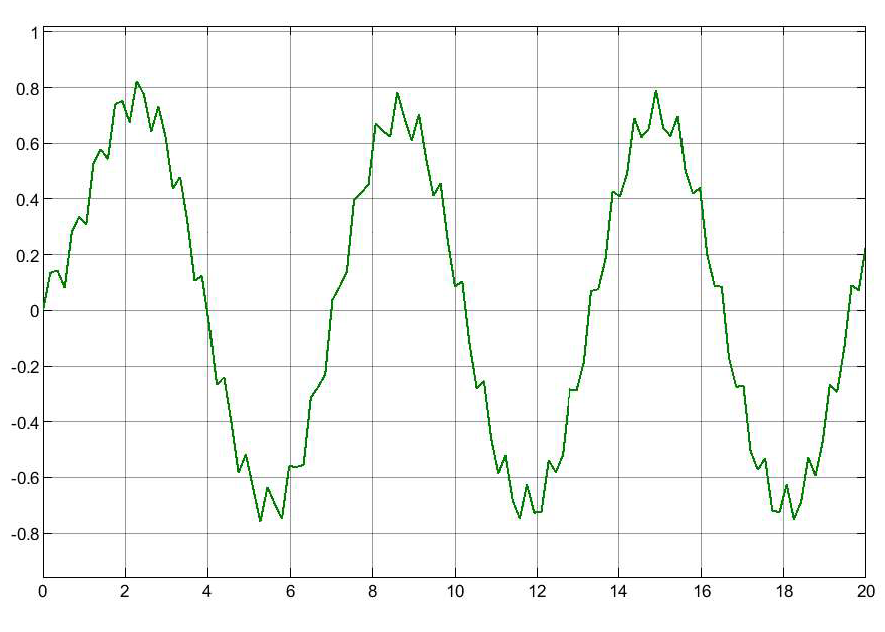
\includegraphics[width=\textwidth]{fig/especifico_2/onda_filtrada.pdf}
        \caption{Onda simulada resultante luego de la función de transferencia}
        \label{fig:onda_filtrada_simulada_matlab}
    \end{subfigure}
    \hfill
    \begin{subfigure}[b]{0.45\textwidth}
        \centering
        \includegraphics[width=\textwidth]{fig/especifico_2/Filtered.pdf}
        \caption{Onda experimental resultante luego de la función de transferencia}
        \label{fig:onda_filtrada_experimental_zedboard}
    \end{subfigure}
    \caption{Comparación de la salida resultante simulada (izquierda) y experimental (derecha)}
    \label{fig:comparacion_salida_resultante}
\end{figure}

Como se pudo observar en la Figura \ref{fig:comparacion_salida_resultante}, a la izquierda se puede observar la gráfica proveniente de la simulación del sistema, por otro lado en la derecha se puede observar la gráfica proveniente de la ejecución del sistema en la tarjeta de desarrollo, estas mediciones corresponden a las señales resultantes luego de la etapa de filtrado del caso de estudio desarrollado en esta sección. 

Para un mejor análisis de resultados se utilizó el código de Python que se muestra en \ref{apx:comparacion_de_sennales_programa}, el cual se encarga de tomar tanto el archivo de salida de la simulación como el archivo de salida del caso experimental y compararlas, esto con el objetivo de poder medir el error promedio absoluto, el error cuadrático medio y la raíz cuadrada del mismo y de esta forma poder cuantificar las diferencias entre la señal de salida simulada y la experimental.

Para este caso de estudio se obtuvieron los siguientes resultados:

\begin{table}[htbp!]
    \centering
    \caption{Precisión de la implementación del caso de estudio 1}
    \label{tab:filter-error}
    \begin{tabular}{ll}
    Métrica                       & Error \\ \hline
    Error promedio absoluto         &   $1.930 \times 10^{-18}$ [V]    \\
    Error cuadrático medio          &   $2.14 \times 10^{-34}$ $[V^{2}]$    \\
    Raíz del error cuadrático medio &   $1.46 \times 10{-17}$ [V]  
    \end{tabular}
    \end{table}


Los valores de error obtenidos son bajos, esto indica un alto nivel de correspondencia entre la señal simulada y la señal experimental. Por un lado tenemos el error promedio absoluto, el cual represente la diferencia promedio entre la simulación y el experimento, al ser esta métrica representada por un valor de $1.930 \times 10^{-18}$ V sugiere que las diferencias entre ambas señales son despreciables. Por otro lado, tenemos el error cuadrático medio, este es asociado con un valor de $2.14 \times 10^{-34}$ $V^{2}$, lo que indica que las desviaciones en las mediciones son mínimas y puntuales. Finalmente la raíz del error cuadrático medio, la cual es representada por el valor de $1.46 \times 10{-17}$ V representa la magnitud promedio de las diferencias cuadráticas. La cercanía a cero que otorga este valor refuerza la alta precisión del modelo en relación con la señal experimental.

Al tener valores tan bajos en las métricas encargadas de medir el error de los modelos se puede respaldar que el proceso experimental es acorde a los resultados de simulación, cumpliendo con los requisitos de exactitud de forma notable.

\section{Reflexión final}

Los resultados de error obtenidos son satisfactorios, lo cual respalda la implementación del caso de estudio realizada a lo largo de este capítulo. Estos valores indican una correspondencia perfecta entre la simulación y el proceso experimental. La alta precisión alcanzada no solo válida el modelo desarrollado, sino que también resalta la consistencia y fiabilidad del proceso experimental. Es por esto que se aprueba el marco de trabajo realizado y se continúa con la investigación del mismo, ya que los porcentajes de error que se muestran en la Tabla \ref{tab:filter-error} respaldan que se logra a cabalidad el establecimiento de un flujo de trabajo para el prototipado de algoritmos de control de orientación y navegación para aplicaciones espaciales.  
